%
% 2-euklid.tex -- Der eudklidische Algorithmus
%
% (c) 2026 Prof Dr Andreas Müller
%
\section{Der euklidische Algorithmus
\label{buch:ratint:section:euklid}}
\kopfrechts{Der euklidische Algorithmus}%
Die Konstruktion der Partialbruchzerlegung hat erfordert, dass gemeinsame
Faktoren von Polynomen gefunden werden mussten.
Es ist natürlich immer denkbar, eine Faktorisierung der beteiligten
Polynome zu suchen, und die gemeinsamen Faktoren zu identifizieren.
Der Fundamentalsatz der Algebra garantiert zwar, dass solche
Faktoren über $\mathbb{C}$ existieren, für die Anwendung in einem
Computeralgebrasystem brauchen wir aber eine Faktorisierung über
$\mathbb{Q}$ oder einer Körpererweiterung von $\mathbb{Q}$, die in
endlich vielen Schritten erreicht werden kann.

Das Finden der Faktoren ist eine weitere Schwierigkeit.
Selbst über $\mathbb{C}$ können die vom Fundamentalsatz garantierten
Linearfaktoren für Polynome vom Grad $\ge 5$ algorithmisch im
Allgemeinen nicht gefunden werden.
Es ist daher nicht angebracht, auf dem Umweg über die Faktorisierung
nach gemeinsame Faktoren zu suchen.

Es gibt aber eine direkte Möglichkeit, gemeinsame Faktoren zu finden.
In seiner ursprünglichen Version, die in
Abschnitt~\ref{buch:ratint:euklid:subsection:ganzezahlen}
beschrieben wird, findet der euklidische Algorithmus den grössten
gemeinsamen Teiler $r$ zweier ganzer Zahlen $a$ und $b$.
Die erweiterte Form ist zudem in der Lage, den grössten gemeinsamen
Teiler als $r=sa+tb$ zu schreiben mit ganzen Zahlen $s,t\in\mathbb{Z}$.
Diese Version kann dazu verwendet werden, die multiplikative Inverse 
in einem endlichen Körper zu finden.

Der euklidische Algorithmus ist nicht auf ganze Zahlen beschränkt.
Er lässt sich in jedem sogenannten euklidischen Ring durchführen.
Dazu gehören auch die Polynomringe.
Der grösste gemeinsame Teiler von zwei Polynomen ist ein gemeinsamer
Faktor, der gemeinsame Nullstellen enthält.
Eine mehrfache Nullstelle eines Polynoms $p(X)$ führt zu einem gemeinsamen
Teiler von $p'(X)$ und $p(X)$.
Solche mehrfache Faktoren können also mit dem euklidischen Algorithmus
gefunden werden.

%
% Der euklidische Algorithmus für ganz Zahlen
%
\subsection{Der euklidische Algorithmus für ganze Zahlen
\label{buch:ratint:euklid:subsection:ganzezahlen}}
In diesem Abschnitt wird der euklidische Algorithmus für ganze
Zahlen entwickelt.
Diese Form des Algorithmus ist seit dem Altertum bekannt und wird
oft bereits in der Mittelschule ein sowohl historisch
wie auch mathematisch bedeutsames Beispiel eines Algorithmus
unterrichtet.
Im Abschnitt~\ref{buch:ratint:euklid:subsection:polynome} wird
der Algorithmus auf Polynome verallgemeinert.

%
% Der Grundalgorithmus
%
\subsubsection{Der Grundalgorithmus}
Seien $a>b$ natürliche Zahlen und $q$ und $r$ so gewählte
natürliche Zahlen, dass $a=bq+r$ mit $r<b$.
Der grösste gemeinsame Teiler $g=\operatorname{ggT}(a,b)$ teilt dann
sowohl $a$ als auch $b$, er muss daher auch $r$ teilen.
Wiederholt man die Rechnung mit $b$ anstelle von $a$ und $r$ anstelle
von $b$ folgt, dass $g$ erneut den Rest teilt.
Da der Rest immer kleiner wird, gibt es einen Moment, bei dem
er erstmals verschwindet.
Der Divisor $b$ ist dann der grösste gemeinsame Teiler.

\begin{beispiel}
\label{buch:ratint:euklid:bsp:euklidzahlen}
Für die Zahlen $a=36$ und $b=28$ ergibt sich die Rechnung
\begin{center}
\input{chapters/060-ratint/fig/tabular-euklid.tex}
\end{center}
aus der man $\operatorname{ggT}(36,28)=4$ ablesen kann.
\end{beispiel}

%
% Der erweiterte Algorithmus
%
\subsubsection{Der erweiterte Algorithmus}
Wir analysieren den euklidischen Algorithmus nochmals etwas im Detail.
Dazu führen wir die folgende Notation ein.
Wir beginnen mit $a_0=a$ und $b_0=b$.
\index{euklidischer Algorithmus!erweitert}%
Wir konstruieren dann $q_0$ und $r_0$ mit $a_0=q_0b_0+r_0$ und 
setzen anschliessend $a_1 = b_0$ und $b_1 = r_0$.
Dieser Prozess wird für $k>0$ gemäss
\begin{align*}
a_k &= b_{k-1} &
b_k &= r_{k-1} &
&\text{und}&
a_k &= q_k b_k + r_k 
&&\Rightarrow&
r_k &= a_k - q_kb_k
\end{align*}
wiederholt, bis $r_{n+1}=0$ ist.
Der grösste gemeinsame Teiler ist dann $r_n$.
Rechnet man ausgehend von $r_n$ rückwärts, findet man
\begin{align*}
r_n &= a_n - q_n b_n
\\
    &= b_{n-1} - q_n r_{n-1}
\\
    &= b_{n-1} - q_n ( a_{n-1} - q_{n-1} b_{n-1} )
     = q_n a_{n-1} + (1 + q_n q_{n-1}) b_{n-1}
\\[-4pt]
    &\phantom{1}\vdots
\intertext{Durch wiederholte Anwendung der Definitionsformeln
für $a_k$ und $b_k$ finden wir schliesslich ganze Zahlen $s$ und $t$
mit der Eigenschaft}
    &= s a_0 + t b_0.
\end{align*}

\begin{beispiel}
Für das Beispiel~\ref{buch:ratint:euklid:bsp:euklidzahlen} folgt
aus der zweiten Zeile der Tabelle
\[
\operatorname{ggT}(a,b)
=
4
= 
28 - 3\cdot 8
\]
Da 8 der Rest der vorangegangenen Zeile ist, kann man ihn durch
$36-1\cdot 28$ ersetzen und erhält
\[
4
=
28 - 3 \cdot (36-28)
=
4\cdot 28 - 3\cdot 36.
\]
Damit sind die Zahlen $s=-3$ und $t=4$ gefunden.
\end{beispiel}

Der erweiterte euklidische Algorithmus kann also nicht nur den 
grössten gemeinsamen Teiler von $a$ und $b$ finden, sondern zusätzlich
Zahlen $s$ und $t$ derart, dass
\[
sa + tb
=
\operatorname{ggT}(a,b)
\]
gilt.
Die Berechnung nach Abschluss ist jedoch eher umständlich.
Gewünscht ist eine Erweiterung des Grundalgorithmus, die die Zahlen
$s$ und $t$ gleich mitberechnet.

\begin{satz}
Gegeben sind die natürlichen Zahlen $a$ und $b$.
Der folgende Algorithmus berechnet den grössten gemeinsamen Teiler $g$
und Zahlen $s$ und $t$ mit $g=sa+tb$.
\begin{enumerate}
\item
Setze $a_0=a$, $b_0=b$, $k=0$ und $s_{-2}=1$, $t_{-2}=0$, $s_{-1}=0$
und $t_{-1}=1$
\item
Finde $q_k$ und $q_k$ mit $a_k= q_kb_k+r_k$.
\item
Berechne
$s_k=s_{k-2}-q_ks_{k-1}$ 
und
$t_k=t_{k-2}-q_kt_{k-1}$.
\end{enumerate}
Für alle $k$ gilt
$r_k = s_ka+t_kb$
Für den grössten Index $n$, für den $r_n\ne 0$ ist, folgt
\[
\operatorname{ggT}(a,b)
=
s_na+t_nb
\qquad\text{und}\qquad
0
=
s_{n+1}a+t_{n+1}b.
\]
\end{satz}

\begin{proof}
Wir schreiben die Division als Matrizenprodukt:
\[
\begin{pmatrix}
b_k\\
r_k
\end{pmatrix}
=
\begin{pmatrix*}[r]
b_k\\
a_k-q_kb_k
\end{pmatrix*}
=
\underbrace{
\begin{pmatrix}
 0 & 1   \\
 1 &-q_k
\end{pmatrix}
}_{\displaystyle = Q(q_k)}
\begin{pmatrix}
a_k\\
b_k
\end{pmatrix}.
\]
Wiederholte Anwendung ergibt
\[
\begin{pmatrix}
r_n\\
0
\end{pmatrix}
=
Q(q_{n+1})
Q(q_n)
\cdots
Q(q_1)
Q(q_0)
\begin{pmatrix}
a\\ b
\end{pmatrix}.
\]
Das Produkt der Matrizen enthält in der ersten Zeile die gesuchten
Zahlen $s_n$ und $t_n$ und in der zweiten Zeile die Zahlen
$s_{n+1}$ und $t_{n+1}$.

Da das Matrizenprodukt assoziativ ist, kann das Produkt von rechts
her aufgelöst werden.
Dazu definieren wir die Matrix
\[
S_k
= 
\begin{pmatrix}
s_{k-1} & t_{k-1} \\
s_{k}   & t_{k} 
\end{pmatrix}
\]
mit der initialen Matrix
\[
S_{-1}
=
\begin{pmatrix}
s_{-2} & t_{-2} \\
s_{-1} & t_{-1} 
\end{pmatrix}
=
\begin{pmatrix}
1 & 0\\
0 & 1
\end{pmatrix}.
\]
Die Multiplikation mit $Q(q_k)$ mit $S_{k-1}$ erzeugt $S_k$, es gilt
daher die Rekursionsformel
\begin{align*}
S_k
&= 
\begin{pmatrix}
s_{k-1} & t_{k-1} \\
s_{k}   & t_{k} 
\end{pmatrix}
=
Q(q_k)
S_{k-1}
=
Q(q_k)
\begin{pmatrix}
s_{k-2} & t_{k-2} \\
s_{k-1} & t_{k-1} 
\end{pmatrix}
\\
&=
\begin{pmatrix}
0&1\\
1&-q_k
\end{pmatrix}
\begin{pmatrix}
s_{k-2} & t_{k-2} \\
s_{k-1} & t_{k-1} 
\end{pmatrix}
\\
&=
\begin{pmatrix*}[r]
s_{k-1}            & t_{k-1}           \\
s_{k-2}-q_ks_{k-1} & t_{k-2}-q_kt_{k-1} 
\end{pmatrix*}.
\end{align*}
In der zweiten Zeile stehen die Rekursionsformeln für die
Zahlen $s_k$ und $t_k$.
\end{proof}

\begin{beispiel}
\label{buch:ratint:euklid:bsp:erweitert}
Wir führen den erweiterten euklidischen Algorithmus für $a=43$ und $b=47$
durch:
\begin{center}
\begin{tabular}{|>{$}r<{$}|>{$}r<{$}>{$}r<{$}|>{$}r<{$}>{$}r<{$}|>{$}r<{$}>{$}r<{$}|}
\hline
  k &  a_k &  b_k &  q_k &  r_k &  s_k &  t_k \\
\hline
 -2 &      &      &      &      &    1 &    0 \\
 -1 &      &      &      &      &    0 &    1 \\
  0 &   43 &   47 &    0 &   43 &    1 &    0 \\
  1 &   47 &   43 &    1 &    4 &   -1 &    1 \\
  2 &   43 &    4 &   10 &    3 &   11 &  -10 \\
  3 &    4 &    3 &    1 &
\smash{\rlap{\raisebox{-14pt}{\begin{tikzpicture}[>=latex,thick]
\fill[color=darkred!20] (0,0) rectangle (2.5,0.8);
\end{tikzpicture}}}}%
                   \phantom{0}1 &  -12 &   11 \\
  4 &    3 &    1 &    3 &    0 &   47 &  -43 \\
\hline
\end{tabular}
\end{center}
In der letzten Zeile wird der Rest $0$, der grösste gemeinsame Teiler ist
also $\operatorname{ggT}(a,b) = r_3=1$.
In der Zeile $k=3$ kann man die beiden Zahlen $s=s_3=-12$ und $t=t_3=11$
ablesen, und tatsächlich ist
\[
-12\cdot 43 + 11\cdot 47 =  1
\qquad\text{und}\qquad
47\cdot 43 - 43\cdot 47 = 0.
\qedhere
\]
\end{beispiel}

Das Beispiel illustriert auch, dass die im Grundalgorithmus formulierte
Bedingung, dass $a>b$ sein muss, unwichtig ist.
Wenn nämlich $a<b$ ist, dann ist der erste Quotient $q_0=0$ und der erste
Rest $r_0=a$.
Daraus ergibt sich dann $a_1=b$ und $b_1=a$, d.~h.~die beiden Zahlen $a$
und $b$ haben die Plätze getauscht.
Auch die Zahlen $s_0=1$ und $t_0=0$ tauschen die Plätze der Anfangsbedingungen
für die Folgen $s_k$ und $t_k$.

%
% Anwendung des erweiterten Algorithmus
%
\subsubsection{Anwendung des erweiterten Algorithmus}
Der erweiterte euklidische Algorithmus kann dazu verwendet werden,
die multiplikative inverse in einem endlichen Körper zu finden.
Sei $p$ eine Primzahl und $\mathbb{F}_p$ die Menge der Reste modulo $p$.
Die multiplikative Inverse eines Elementes $a\in\mathbb{F}_p$ kann
jetzt wie folgt gefunden werden.
Da $p$ ein Primzahl ist, sind $a$ und $p$ teilerfremd.
Der erweiterte euklidische Algorithmus liefert zwei Zahlen $s$ und $t$
mit
\[
sa + tp = \operatorname{ggT}(a,p) = 1.
\]
Modulo $p$ wird diese Gleichung zu
\[
sa \equiv 1 \mod p.
\]
Der Rest von $s$ modulo $p$ ist daher die multiplikative Inverse $a$.

\begin{beispiel}
Für $p=47$ und $a=43$ ergibt der in
Beispiel~\ref{buch:ratint:euklid:bsp:erweitert}
durchgeführte, erweiterte euklidische Algorithmus
\[
-12 \cdot 43
+
11\cdot 47
= 1.
\]
Die multiplikative Inverse von $43$ im Körper $\mathbb{F}_{47}$ ist
daher $-12\equiv 35\mod 47$.
\index{multiplikative Inverse in F_p@multiplikative Inverse in $\mathbb{F}_p$}%
Tatsächlich ist 
\[
35\cdot 43 = 1505 = 32\cdot 47 + 1,
\]
wie behauptet.
\end{beispiel}


%
% 22-polynome.tex -- Der euklidische Algorithmus für Polynome
%
% (c) 2026 Prof Dr Andreas Müller
%
\subsection{Der euklidische Algorithmus für Polynome
\label{buch:ratint:euklid:subsection:polynome}}
Der euklidische Algorithmus funktioniert auch für Polynome.
Dies ermöglicht, rationale Funktionen effizient zu kürzen.
Später werden wir den erweiterten euklidischen Algorithmus
auch verwenden, um die quadratfreie Faktorisierung und die 
zugehörige Partialbruchzerlegung einer rationalen Funktion
zu finden und um Integrale von rationalen Funktionen auf 
einfachere Form zu reduzieren.

%
% Polynomdivision
%
\subsubsection{Polynomdivision}
Auch für Polynome gibt es eine Division mit Rest.
Zu zwei Polynomen $a(x)$ und $b(x)$ gibt es Polynome $q(x)$ und $r(x)$,
für die
\[
a(x) = b(x)q(x)+r(x)
\]
gilt.
Ausserdem muss der Grad des Restpolynoms $r(x)$ kleiner sein als
der Grad von $b(x)$: $\deg r(x) < \deg b()$.

\begin{beispiel}
\label{buch:ratint:euklid:bsp:polynomdivision}
Der Divisionsalgorithmus liefert für die Polynome
\[
a(x)
=
x^4+x^3-4x^2+x-6
\qquad\text{und}\qquad
b(x)
=
x^2+5x+6
\]
die folgende Rechnung:
\[
\renewcommand{\arraycolsep}{1.2pt}
\begin{array}{rcrcrcrcrcrcrcrcrcrcr}
x^4&+&  x^3&-& 5x^2&+&  x&-& 6&:& x^2&+& 5x&+& 6 &=& x^2 &-& 4x&+& 9\\
x^4&+& 5x^3&+& 6x^2& &   & &  & &    & &   & &   & &     & &   & &  \\
\cline{1-5}
   &-& 4x^3&-&11x^2&+&  x& &  & &    & &   & &   & &     & &   & &  \raisebox{4pt}{\mathstrut}\\
   &-& 4x^3&-&20x^2&-&24x& &  & &    & &   & &   & &     & &   & &  \\
\cline{2-7}
   & &     & & 9x^2&+&25x&-& 6& &    & &   & &   & &     & &   & &  \raisebox{4pt}{\mathstrut}\\
   & &     & & 9x^2&+&45x&+&54& &    & &   & &   & &     & &   & &  \\
\cline{5-9}
   & &     & &     &-&20x&-&60& &    & &   & &   & &     & &   & &  \raisebox{3pt}{\mathstrut}\\
\cline{6-9}
\end{array}
\]
Somit ist der Quotient $q(x)=x^2-4x+9$ und der Rest $r(x)=-20x-60$.
\end{beispiel}

Die Division von Polynomen ist die Basis des Algorithmus zur Bestimmung
des grössten gemeinsamen Teilers.
Es ist aber zu beachten, dass die Division einen Rest liefert,
der nicht unbedingt ein normiertes Polynom ist.
Es kann daher nötig sein, den Rest zu normieren.
Im Beispiel ist der normierte Rest $x+3$.

%
% Gemeinsame Teiler für Polynome
%
\subsubsection{Gemeinsame Teiler für Polynome}
Der euklidische Algorithmus für den grössten gemeinsamen Teiler
funktioniert unverändert auch für Polynome.
Der Polynomgrad des Restes nimmt dabei ständig ab, bis der Rest
0 wird.

\begin{beispiel}
Man finde den grössten gemeinsamen Teiler der Polynome
\[
a(x)
=
x^4+x^3-5x^2+x-6
\qquad\text{und}\qquad
b(x)
=
x^2+5x+6.
\]
Dazu müssen die Quotienten und Reste berechnet werden, der
erste wurde bereits im
Beispiel~\ref{buch:ratint:euklid:bsp:polynomdivision}
berechnet:
\begin{center}
\begin{tabular}{|>{$}r<{$}|>{$}l<{$}>{$}l<{$}|>{$}l<{$}>{$}l<{$}|}
\hline
 k & a_k              & b_k      & q_k                & r_k
\raisebox{2.5pt}{\mathstrut}\\[1pt]
\hline
 0 & x^4+x^3-5x^2+x-6 & x^2+5x+6 & x^2-4x+9           & -20x-60
\raisebox{3pt}{\mathstrut}\\
 1 & x^2+5x+6         & -20x-60  & -\frac{1}{20}(x+2) &       0
\\[2pt]
\hline
\end{tabular}
\end{center}
In der zweiten Zeile lässt sich ablesen, dass der Rest $=0$ ist,
daher ist der grösste gemeinsame Teiler $-20x-60$.
Dieses Polynom ist nicht normiert, da die Koeffizienten rational sind,
kann man durch $-20$ teilen und erhält das normierte Polynom $x+3$.
\end{beispiel}

Das Beispiel zeigt auch, dass der gefundene grösste gemeinsame Teiler
nicht ein normiertes Polynom ist.
Da wir nur an Polynomen mit rationalen Koeffizienten interessiert
sind, kann immer durch den Leitkoeffizient geteilt werden.
Arbeitet man dagegen nur mit ganzzahligen Koeffizienten, wird im 
Beispiel bereits der Schritt $k=2$ nicht mehr durchführbar.

%
% Der erweiterte euklidische Algorithmus für Polynome
%
\subsubsection{Der erweiterte euklidische Algorithmus für Polynome}
Auch der erweiterte euklidische Algorithmus lässt sich übertragen.

\begin{beispiel}
Für die Polynome $a(x) = x^3+2x^2-x-2$ und $b(x)=x^2-x-2$
finde man Polynome $s(x)$ und $t(x)$ mit
$\operatorname{ggT}(a,b)=s(x)a(x)+t(x)b(x)$.
\begin{center}
\renewcommand{\arraycolsep}{1.2pt}
\begin{tabular}{|>{$}r<{$}|>{$}l<{$}>{$}l<{$}|>{$}l<{$}>{$}l<{$}|>{$}l<{$}>{$}l<{$}|}
\hline
  k & a_k(x)        & b_k(x)  & q_k(x)       & r_k(x) & s_k(x) & t_k(x) \raisebox{2.5pt}{\mathstrut}\\[1pt]
\hline
 -1 &               &         &              &        &             1 &                0 \\
 -2 &               &         &              &        &             0 &                1 \\
  0 & x^3+2x^2-2x-2 & x^2-x-2 & x+3          & 4x + 4 &             1 &             -x-3 \\
  1 & x^2-x-2       & 4x+4    & \frac14(x-2) & 0      & -\frac14(x-2) & \frac14(x^2+x-2) \\[2pt]
\hline
\end{tabular}
\end{center}
Tatsächlich können wir nachrechnen, dass
\begin{align*}
s_0(x)
\cdot
a(x)
+
t_0(x)
\cdot
b(x)
&=
1
\cdot
(x^3+2x^2-x-2)
-
(x+3)
\cdot
(x^2-x-2)
\\
&=
(x^3+2x^2-x-2)
-
(x^3+2x^2-5x-6)
\\
&=
4x+4
\intertext{und}
s_1(x)
\cdot
a(x)
+
t_1(x)
\cdot
b(x)
&=
-
\frac14(x-2)
\cdot
(x^3+2x^2-x-2)
+
\frac14(x^2+x-2)
\cdot
(x^2-x-2)
\\
&=
-
\frac14(x^4-5x^2+4)
+
\frac14(x^4-5x^2+4)
\\
&=0.
\end{align*}
Verlangt man ein normiertes Polynom für den grössten gemeinsamen Teiler,
kann man die Koeffizienten in $\mathbb{Q}$ durch $4$ dividieren und 
erhält $\operatorname{ggT}(a,b)=x+1$.
Die Faktoren $s(x)$ und $t(x)$ müssen ebenfalls durch 4 geteilt werden
und es gilt
\[
\frac14
\cdot
(x^3+2x^2-x-2)
-\frac14(x+3)
(x^2-x-2)
=
x+1.
\]

Den grössten gemeinsamen Teiler kann man auch mithilfe der Faktorisierung
\begin{align*}
a(x)
&=
(x-1){\color{darkred}(x+1)}(x+2)
\\
b(x)
&=
(x-2){\color{darkred}(x+1)}
\end{align*}
der Polynome finden.
Der einzige gemeinsame Faktor ist $\operatorname{ggT}(a,b)={\color{darkred}x+1}$.
Aus der Faktorisierung sind jedoch die Faktoren $s(x)$ unt $t(x)$
nicht direkt ablesbar.
\end{beispiel}


%
% 23-eudklidisch.tex -- Euklidische Ringe
%
% (c) 2026 Prof Dr Andreas Müller
%
\subsection{Euklidische Ringe
\label{buch:ratint:euklid:subsection:ringe}}
Der euklidische Algorithmus benötigt erst mal, dass es keine
pathologischen Faktoren gibt, die ein Produkt auslöschen können.
Solche pathologischen Fälle führen dazu, dass es nicht sinnvoll ist
von einer eindeutigen Faktorisierung zu sprechen.
Pathologische Faktoren heissen Nullteiler im Sinne der folgenden
Definition.

\begin{definition}[Nullteiler, Integritätsbereich]
Nullteiler \emph{Nullteiler} in einem Ring $R$ sind Zahlen
$a,b\in R^*=R\setminus\{0\}$ mit $ab=0$.
Ein Ring $R$ ohne Nullteiler heisst \emph{nullteilerfrei} oder ein
\emph{Integritätsbereich}.
\index{Nullteiler}%
\index{nullteilerfrei}%
\index{Integritatsbereich@Integritätsbereich}%
\end{definition}

Die ganzen Zahlen und die Menge der Polynome bilden Integritätsbereiche.

Der euklidische Algorithmus für ganze Zahlen verwendet, dass der Rest
bei der ganzzahligen Division kleiner als der Divisor ist.
Polynome kann man nicht vergleichen.
Der euklidische Algorithmus für Polynome braucht aber, dass der Grad
des Restes kleiner wird als der Grad des Divisors.
Der Algorithmus ist also auf eine allgemeinere Situation übertragbar,
wenn ein Eigenschaft ähnlich dem Grad gefunden werden kann, die bei
der Division kleiner wird.

\begin{definition}[Euklidischer Ring]
\label{buch:ratint:euklid:def:euklidischerring}
Ein nullteilerfreier Ring  $R$ heisst ein \emph{euklidischer Ring},
\index{euklidischer Ring}%
\index{Ring!euklidisch}%
wenn es eine Funktion $d\colon R^*\to\mathbb{Z}$
\begin{enumerate}
\item $d(r) \ge 0$ für alle $r\in R^*$.
\item $d(r)\le d(rs)$ für alle $r,s\in R^*$.
\item Sind $a,b\in R^*$, dann gibt es $q,r$ mit $a=qb+r$ mit $r=0$ oder
$d(r)<d(b)$.
\end{enumerate}
Die Funktion $d$ heisst auch die \emph{Gradfunktion} des euklidischen
Rings.
\index{Gradfunktion}%
Die letzte Eigenschaft kann etwas vereinfacht werden, wenn man
$d(0)=-\infty$ definiert.
\end{definition}

Für die ganzen Zahlen ist die $d\colon\mathbb{Z}^*\to\mathbb{Z}: a\to a$
die Funktion, die die ganzen Zahlen zu einem euklidischen Ring macht.
Für Polynome mit Koeffizienten in einem Körper ist es der Grad
$\deg\colon K[X] \to \mathbb{Z} : p(X) \mapsto \deg p$.

Ein weiteres interessantes Beispiel für einen euklidischen Ring ist
der Ring der ganzen gaussschen Zahlen.

\begin{beispiel}
Wir betrachten die Menge
\[
\mathbb{Z}[i]
=
\{a+bi\mid a,b\in\mathbb{Z}\}\subset\mathbb{C}.
\]
Sie heisst der \emph{Ring der ganzen gaussschen Zahlen}.
\index{ganze gausssche Zahlen}%
\index{gausssche Zahlen}%
Als Teilmenge des Körpers der komplexen Zahlen ist $\mathbb{Z}[i]$
sicher ein nullteilerfreier Ring.
Als Gradfunktion kann das Betragsquadrat 
\[
d
\colon
\mathbb{Z}[i] \to \mathbb{Z}
:
(a+bi) \mapsto a^2+b^2
\]
verwendet werden.
Es müssen die drei Eigenschaften der 
Definition~\ref{buch:ratint:euklid:def:euklidischerring}
verifizieren.
\begin{enumerate}
\item
Für $a+bi\ne 0$ ist $d(a+bi)=a^2+b^2>0$.
\item
Für das Produkt gilt für $(a+bi)\ne 0$ ist $d(a+bi)\ge 1$
\[
d\bigl(
(a+bi)(c+di)
\bigr)
=
(a^2+b^2)(c^2+d^2)
=
d(a+bi)d(c+di)
\ge
d(c+di)
\]
für all $c+di\in \mathbb{Z}[i]$.
\item
Diese Eigenschaft wird am einfachsten auf die folgende geometrische
Weise verständlich (Abbildung~\ref{buch:ratint:euklid:fig:ggz}).
%
% fig-ggz.tex -- eukldische Eigenschaft für ganze gaussche Zahlen
%
% (c) 2026 Prof Dr Andreas Müller
%
\begin{figure}
\centering
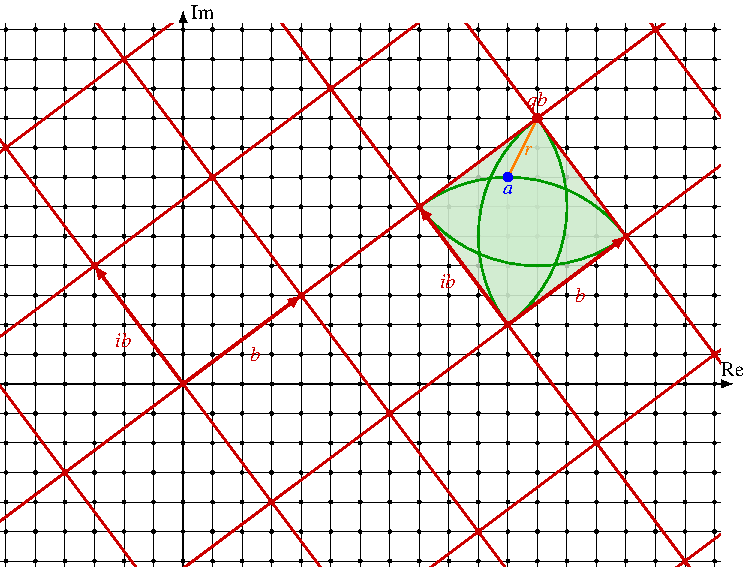
\includegraphics{chapters/060-ratint/images/ggz.pdf}
\caption{Euklidische Eigenschaft des Rings der ganzen gaussschen Zahlen.
Die Vielfachen $\mathbb{Z}[i]b= \{xb+y ib\mid x,y\in\mathbb{Z}\}$
bilden ein quadratisches Gitter ({\color{darkred}rot}). 
Die Zahl $a$ ({\color{blue}blau}) muss in einem der Gitterquadrate
({\color{darkgreen}grün}) liegen, die Seitenkanten $b$ und $ib$ haben.
Da die Kreise mit Radius $|b|$ um die Ecken das ganze Quadrat überdecken,
gibt es eine Ecke, die näher an $a$ ist als $|b|$.
Mit dem $q=x+iy$ dieser Ecke folgt $r=a-qb$ und $|r|<|b|$
bzw.~$d(r) = |r|^2 < |b|^2=d(b)$.
\label{buch:ratint:euklid:fig:ggz}}
\end{figure}
%
Die Menge 
\[
b\mathbb{Z}[i]
=
\{ zb\mid z \in \mathbb{Z}[i] \}
=
\{ xb + iyb \mid x,y\in \mathbb{Z}
\}
\]
bildet ein Gitter in der komplexen Zahlenebene.
Da $b$ und $ib$ senkrecht aufeinander stehende Vektoren sind, 
handelt es sich um ein quadratisches Gitter.
Der Punkt $a$ muss in einem der Gitterquadrate liegen.
Jede Ecke dieses Quadrats wird durch ein $q\in\mathbb{Z}[i]$
beschrieben und kommt als das $q$ in der Eigenschaft~3 eines eukldischen
Rings in Frage.
Die zusätzliche Forderung $d(r)<d(b)$ bedeutet, dass der Punkt $a$
näher als die Kantenlänge des Quadrates bei der ausgewählten Ecke
sein muss.
Da die offenen Kreisscheiben mit Radius $|b|$ die Quadratfläche 
vollständig überdecken, muss es mindestens ein $q\in\mathbb{Z}[i]$
(eine Ecke) geben,
so dass $a-qb=r$ die Bedingung $d(r) < d(b)$ ($|r|<|b|$) erfüllt ist.
\end{enumerate}
Dies zeigt, dass die ganzen gaussschen Zahlen einen euklidischen
Ring bilden.
Es ist daher sinnvoll, vom grössten gemeinsamen Teiler ganzer
gaussscher Zahlen zu sprechen und es ist möglich, diese mit dem
euklidischen Algorithmus zu finden.
\end{beispiel}

Die ganzen gaussschen Zahlen können zum Beispiel dazu verwendet
werden, dann folgenden fermatschen Zweiquadratesatz zu beweisen
\cite[Satz 10.4]{buch:luneburg}.

\begin{satz}[Fermat]
\index{Fermat, Pierre de}%
\index{Satz!von Fermat}%
Ist $p$ eine Primzahl mit $p\equiv 1\mod 4$, dann gibt es ganze
Zahlen $a,b\in\mathbb{Z}$ mit $p=a^2+b^2$.
\end{satz}




%
% 24-koerper.tex -- Körperkoeffizienten
%
% (c) 2026 Prof Dr Andreas Müller
%
\subsection{Polynome mit Koeffizienten in einem beliebigen Körper}
Der euklidische Algorithmus, wie er in
Abschnitt~\ref{buch:ratint:euklid:subsection:polynome}
für Polynome mit Koeffizienten in $\mathbb{Q}$ oder $\mathbb{C}$
vorstellt wurde, ist in keiner Weise auf solche Zahlkörper beschränkt.
Damit die Polynomdivision und damit die Bestimmung des Rests
in jedem Schritt des euklidischen Algorithmus durchgeführt werden kann,
ist nur nötig, dass die Koeffizienten aus einem Körper stammen.
Die Diskussion der Eigenschaften euklidischer Ringe in
Abschnitt~\ref{buch:ratint:euklid:subsection:ringe} hat dies
gezeigt.

Ist $K$ ein Körper, dann ist auch die Menge $F=K(x)$ der rationalen Funktionen
in der Variablen $x$ ein Körper.
$F$ ist ein euklidischer Ring.
Für Polynome mit Koeffizienten in $F$ gilt daher ebenfalls der
euklidische Algorithmus.

Eine Funktion wie
\[
f(z)
=
\frac{2z\log z + 9}{\frac1z-\log z}
\]
kann als rationale Funktion in der Variablen $\vartheta=\log z$
mit Koeffizienten im Körper $\mathbb{Q}(z)$ der rationalen Funktionen
in der Variablen $z$ betrachtet werden.
Zähler und Nenner sind Polynome
\[
2z\vartheta + 9
\qquad\text{und}\qquad
\frac1z -\vartheta
\]
in $\vartheta$ mit rationalen Funktionen als Koeffizienten.
Die Schreibweise
\[
f(z)
=
\frac{2z\vartheta - 9}{\frac1z-\vartheta}
\]
mit $\vartheta$ macht dies deutlich.
Wir werden dies im Kapitel~\ref{chapter:intalg} wiederholt ausnutzen,
um einen Integrationsalgorithmus zu konstruieren.
Wir werden dazu den Grundkörper der rationalen Funktionen in $z$ 
durch weitere Funktionen wie $\vartheta$ erweitern.
Die Erweiterung verlangt nur, dass wir mit rationalen Funktionen
umgehen können müssen.
Zwar ergeben sich zusätzliche Erschwernisse dadurch, dass die Koeffizienten
nicht konstant sind, aber die prinzipielle Vorgehensweise von
Abschnitt~\ref{buch:ratint:bernoulli:subsection:prinzip}
bleibt gültig.




